
\chapter{Functors}

If in order to study groups, modules or topological spaces, one should study the homomorphisms or continuous maps between them, then to study categories one should study `morphisms of categories'. Such morphisms of categories are called \emph{functors}. 

\section{Definition of a functor}

\begin{definition} Let $\cC$ and $\cD$ be categories. A \emph{functor} $F$ from $\cC$ to $\cD$, consists of the data of
\begin{enumerate}
\item for every object $X$ in $\cC$ an object $F(X)$ in $\cD$,
\item for every morphism $f\colon X\to Y$ in $\cC$ a morphism $F(f)\colon F(X) \to F(Y)$ in $\cD$
\end{enumerate}
subject to the conditions
\begin{enumerate}
\item[(F1)] for every $X$ in $\cC$ we have $F(\id_X) = \id_{F(X)}$
\item[(F2)] for every $f\colon X\to Y$ and $g\colon Y\to Z$ in $\cC$ we have $F(gf)=F(g)F(f)$.
\end{enumerate}
\end{definition}

We will  write $F\colon \cC\to \cD$ to denote that $F$ is a functor from $\cC$ to $\cD$.

Note that if $F\colon \cC\to \cD$ and $G\colon \cD \to \cE$ are functors, then  the composite $GF\colon \cC \to \cE$ defined by $(GF)(X) := G(F(X))$ and $(GF)(f) := G(F(f))$ is also a functor. 

To avoid overloading notation, we will often write $FX$ and $Ff$ instead of $F(X)$ and $F(f)$.

\section{Many examples}

\begin{example}[Identity]
For every category $\cC$  there is an identity functor
$\id_\cC \colon \cC \to \cC$ with $\id_\cC(X) = X$ and $\id_\cC(f)= f$. 
\end{example}

\begin{example}[Forgetful functors]\label{exa:forgetful}
Let $R$ be a ring. Then we have a functor
\[
	F\colon {}_R\Mod \to \Ab
\]
defined by $F(M):=M$ (as an abelian group) and $F(f):=f$. 
An $R$-module $M$ is an abelian group equipped with extra structure, and this functor `forgets' the extra structure. Other examples of forgetful functors are the obvious functors $\Top \to \Set$ (forgetting the topology), $\Ab \to \Set$ (forgetting the addition), and $\Ring \to \Ab$ (forgetting the multiplication).
\end{example}
 
\begin{example}[Hom functor]\label{exa:covariant-hom-functor}
Let $\cC$ be a category in which the $\Hom$ classes are sets, and let $X$ be an object of $\cC$. Then we define a functor $F\colon \cC\to \Set$ as follows. For an object $Y$ in $\cC$ we define
\[
	F(Y) := \Hom_\cC(X,Y),
\]
and for a morphism $f\colon Y_1 \to Y_2$ in $\cC$ we define
\[
	F(f) \colon \Hom_\cC(X,Y_1) \to \Hom_\cC(X,Y_2),\, g \mapsto fg.
\]
One easily checks that $F$ is a functor. We  will denote it by $\Hom_\cC(X,-)$.
\end{example}


\begin{example}[Abelianization of a group]\label{exa:abelianization}
If $G$ is a group then we denote by $[G,G]$ its commutator subgroup. This is the subgroup generated by the elements $sts^{-1}t^{-1}$ with $s,t\in G$. It is a normal subgroup, and the quotient group
\[
	G^{\ab} := G/[G,G]
\]
is abelian. It is called the \emph{abelianization} of $G$. If $f\colon G\to H$ is a group homomorphism, then $f([G,G]) \subset [H,H]$,  hence $f$ induces a group homomorphism 
\[
	f^\ab \colon G^\ab \to H^\ab.
\]
Together, these constructions define a functor $(-)^\ab\colon \Grp\to\Ab$.
\end{example}

\begin{example}[Free module]\label{exa:free-module-functor}
Let $R$ be a ring. For every set $I$ we have the free module 
\[
	R^{(I)} := \left\{ (x_i)_{i\in I} \in R^I \mid \text{$x_i=0$ for all but finitely many $i$} \right\},
\]
see Example \ref{ex:free-module}. If $f\colon I\to J$ is a map of sets, then we have an induced map
$R^{(I)} \to R^{(J)}$ 
determined by requiring that $f$ maps the standard basis vector $e_i$ of $R^{(I)}$ to the standard basis vector $e'_{f(i)}$ of $R^{(J)}$. This construction defines a functor $\Set \to {}_R\Mod$.
\end{example}



\begin{example}[The fundamental group of a pointed space] Let $\Top_\ast$ be the category of \emph{pointed topological spaces}. Objects in $\Top_\ast$ are pairs $(X,x)$ with $X$ a topological space and $x\in X$. A morphism from $(X,x)$ to $(Y,y)$ is a continuous map $f\colon X\to Y$ such that $f(x)=y$.

Then the fundamental group defines a functor
\[
	\pi_1\colon \Top_\ast \to \Grp.
\]
On the level of objects it is simply defined by mapping a pair $(X,x)$ to the fundamental group $\pi_1(X,x)$. On the level of morphisms
it is defined as follows. Let $(X,x)$ and $(Y,y)$ be pointed spaces, and let $f \colon X\to Y$ be a continuous map such that $f(x)=y$. Then
we defined $\pi_1(f)$ by
\[
	\pi_1(f) \colon \pi_1(X,x) \to \pi_1(Y,y),\, [\gamma] \mapsto [f\circ \gamma],
\]
where $[\gamma]$ denotes the class of a loop $\gamma\colon [0,1] \mapsto X$ based at $x$.
\end{example} 

Note that the definition of fundamental group requires a base point. Although for a path-connected space $X$ and points $x,y\in X$ the fundamental groups $\pi_1(X,x)$ and $\pi_1(X,y)$ are isomorphic,
the isomorphism is not unique, as it depends on the choice of a path. 
%See also Exercise \ref{exc:fundamental-group-requires-base-point}.


\begin{example}[Solutions to polynomial equations]\label{exa:pol-eq}
Let $f_1,\ldots, f_m \in \bZ[X_1,\ldots, X_n]$. Then we can consider
solutions to the system of polynomial equations $f_1=f_2=\cdots =f_m=0$ in arbitrary commutative rings. Varying the commutative ring, one obtains a functor
\[
	F\colon \CRing \to \Set
\]
defined on the level of objects by  
\[
	R \mapsto \{ x=(x_1,\ldots, x_n) \in R^n \mid f_1(x)=f_2(x)=\cdots =f_m(x) =0 \}.
\]
and on the level of morphisms by 
\[
	\big[ \varphi\colon R\to S\big] \mapsto \big[ (x_1,\ldots,x_n) \mapsto 
	(\varphi(x_1),\ldots,\varphi(x_n))\big].
\]
Indeed, if $\varphi\colon R\to S$ is a ring homomorphism, and if $x\in R^n$ is a solution to the system of equations, then also $(\varphi(x_1),\ldots, \varphi(x_n) ) \in S^n$ is a solution to the system of equations.
\end{example}

\begin{example}[Commutative diagrams as functors] \label{exa:diagrams-as-functors}
Let $\cC$ be the small category 
\[
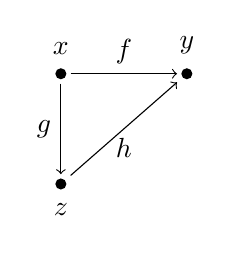
\begin{tikzpicture}
 \node (X) [label=above:{$x$}] at (-.8,.8) {};
 \fill (X) circle[radius=2pt];
 \node (Y) [label=above:{$y$}] at (.8,.8) {};
 \fill (Y) circle[radius=2pt];
 \node (Z) [label=below:{$z$}] at (-.8,-.6) {};
 \fill (Z) circle[radius=2pt];
 
%  \path (X) edge [loop left, out=-150,in=150,min distance=7mm, ->] node {$\id_x$} (X);
%  \path (Y) edge  [loop right, out=30,in=-30,min distance=7mm, ->] node {$\id_y$} (Y);
%  \path (Z) edge  [loop right, out=150,in=210,min distance=7mm, ->] node[left] {$\id_z$} (Z);
   \path (X) edge [->] node[above] {$f$} (Y);
   \path (X) edge [->] node[left] {$g$} (Z);
   \path (Z) edge [->] node[below] {$h$} (Y);
\end{tikzpicture}
\]
with $f=hg$ (and where we omitted $\id_x$, $\id_y$ and $\id_z$ from the picture). Let $\cD$ be any category. Then a functor $F\colon \cC \to \cD$ consists of objects $X:=F(x)$, $Y:=F(y)$, $Z := F(z)$ together with morphisms $F(f)$, $F(g)$ and $F(h)$ between them, such that $F(f)=F(h)F(g)$. In other words, a functor $F\colon \cC \to \cD$ is the same as a triangular commutative diagram
 \[
\begin{tikzcd}
X \arrow{r} \arrow{d} & Y  \\
Z \arrow{ru} 
\end{tikzcd}
\]
in the category $\cD$. With a similar construction, a commutative diagram  in $\cD$ of any shape can be thought of as a functor from some small category $\cC$ to $\cD$.
\end{example}

\section{Contravariant functors}

\begin{definition}
Let $\cC$ and $\cD$ be categories. A \emph{contravariant functor} from $\cC$ to $\cD$ consists of the
data of
\begin{enumerate}
\item for every object $X$ in $\cC$ an object $F(X)$ in $\cD$,
\item for every morphism $f\colon X\to Y$ in $\cC$ a morphism $F(f)\colon F(Y) \to F(X)$ in $\cD$
\end{enumerate}
subject to the conditions
\begin{enumerate}
\item[(F1)] for every $X$ in $\cC$ we have $F(\id_X) = \id_{F(X)}$
\item[(F2')] for every $f\colon X\to Y$ and $g\colon Y\to Z$ in $\cC$ we have $F(gf)=F(f)F(g)$.
\end{enumerate}
\end{definition}

To stress the difference, one sometimes calls an ordinary functor a \emph{covariant functor}.


\begin{remark}
The only difference with the notion of a functor is that $F$ reverses the order of composition. In other words, a contravariant functor $F$ from $\cC$ to $\cD$ is the same as a functor $F\colon \cC^\opp \to \cD$. 

To avoid clashing notation, we will reserve the notation $F\colon \cC \to \cD$ for a functor from $\cC$ to $\cD$, and will write $F\colon \cC^\opp \to \cD$ for a contravariant functor from $\cC$ to $\cD$.
\end{remark}

\begin{example}[Contravariant Hom functor]\label{exa:contravariant-hom-functor}
Let $\cC$ be a category and $X$ an object of $\cC$. If $f\colon Y_1\to Y_2$ is a morphism in $\cC$, then we have an induced map of 
sets
\[
	\Hom_\cC(Y_2,X) \to \Hom_\cC(Y_1,X),\, g \mapsto gf,
\]
and varying $Y$ we obtain a contravariant functor from $\cC$ to $\Set$ given by
\[
	\Hom_\cC(-,X)\colon \cC^\opp \to \Set,\,Y \mapsto \Hom_\cC(Y,X).
\]
This is a contravariant variation on Example \ref{exa:covariant-hom-functor}.
\end{example}

\begin{example}
Another (related) example of a contravariant functor is the `dual vector space'
\[
	(-)^\vee\colon \Vec_K^\opp \to \Vec_K
\]
which maps a $K$-vector space $V$ to its dual $V^{\vee} := \Hom_K(V,K)$ and a linear map
$f\colon V\to W$ to the induced map
\[
	f^\vee\colon W^\vee \to V^\vee,\,
	\varphi \mapsto \varphi\circ f.
\]
\end{example}

\begin{example}[Ring of functions on a space]\label{exa:functions-on-a-space}
Yet another (related) example is the functor
\[
	C\colon \Top^\opp \to \CRing,\, X \mapsto C(X) = \{ \varphi\colon X\to \bR \mid \text{$\varphi$ continuous} \},
\]
mapping a topological space $X$ to the ring of continuous $\bR$-valued functions on $X$ (with point-wise addition and multiplication). On the level of maps it is defined as follows: if $f\colon X\to Y$ is continuous, then we have an induced map
\[
	C(f) \colon C(Y) \to C(X),\, \varphi \mapsto \varphi\circ f,
\]
which is clearly a ring homomorphism. 
\end{example}

\section{Functors with multiple arguments}


It is sometimes useful to consider functors with multiple arguments, living in various categories. This can easily be formalized using the notion of product category (see Definition \ref{def:product-category}). For example, a functor
\[
	F\colon \cC_1 \times \cC_2 \to \cD
\]
assigns to any pair of objects $(X_1,X_2)$ with $X_i\in \ob \cC_i$ an object $F(X_1,X_2)$ in $\cD$, and to any pair of morphisms $(f_1,f_2)$ with $f_i\colon X_i\to Y_i$ in $\cC_i$ a morphism $F(f_1,f_2) \colon F(X_1,X_2) \to F(Y_1,Y_2)$ in $\cD$. 

This can be combined with the notion of a contravariant functor. 

\begin{example}\label{exa:hom-in-two-arguments}
A typical example is the functor
\[
	\Hom_\cC(-,-) \colon \cC^\opp \times \cC \to \Set,
\]
which can be defined for any locally small category $\cC$. If $f\colon X'\to X$ and $g\colon Y\to Y'$ are morphisms in $\cC$ (take note of the directions of the arrows), then we have an induced morphism
\[	
	\Hom_\cC(X,Y) \to \Hom_\cC(X',Y'),
\]
which is given by $\alpha \mapsto g\alpha f$. One says that $\Hom_\cC(-,-)$ is contravariant in the first, and covariant in the second argument.
\end{example}





\newpage
\section*{Exercises}



\begin{exercise}
Let $\cC$ and $\cD$ be categories, let $F\colon \cC \to \cD$ be a functor. Let $f$ be an isomorphism in $\cC$. Show that $F(f)$ is an isomorphism
in~$\cD$.  Give an example where $F(f)$ is an isomorphism but $f$ is not.
\end{exercise}

\begin{exercise}
Verify that if $f\colon R\to S$ is a ring homomorphism, then $f$ restricts to a group homomorphism $R^\times \to S^\times$. Use this to construct a functor $\Ring \to \Grp$, mapping a ring $R$ to its group of units $R^\times$.
\end{exercise}


\begin{exercise}Verify the claims in Example \ref{exa:abelianization}.
\end{exercise}

\begin{exercise}
Let $S$ and $T$ be pre-ordered sets, defining categories $\cC$ and $\cD$ respectively (see Example \ref{exa:pre-ordered}). Describe the functors from $\cC$ to~$\cD$.
\end{exercise}

\begin{exercise}\label{exc:functor-GLn}
For a non-negative integer $n$ we denote by $\GL_n(R)$ the group of invertible $n$ by $n$ matrices with entries in $R$. In other words, the group of units in the ring $\Mat_n(R)$. For example $\GL_1(R) = R^\times$.

Show that $\GL_n$ defines a functor from the category of commutative rings $\CRing$ to the category of groups $\Grp$. 
\end{exercise}


\begin{exercise}[Center is not a functor\ldots]
Show that there exist morphisms $f\colon S_2 \to S_3$ and $g\colon S_3 \to S_2$ in $\Grp$ with the property that $gf=\id_{S_2}$.
Deduce that there is no functor $F\colon \Grp \to \Ab$ such that for every group $G$ we have that $FG$ is isomorphic to the center of $G$.
\end{exercise}

\begin{exercise}[\ldots but it is when we restrict to isomorphisms]
Let $\Grp^\times$ be the category whose objects are groups, and whose morphisms are \emph{isomorphisms} of groups (see also Exercise \ref{exc:iso-category}). Show that there is a functor $Z\colon \Grp^\times \to \Ab^\times$ that maps
a group $G$ to its center.
\end{exercise}
%
%\begin{exercise}[Fundamental group requires a base point\ldots]\label{exc:fundamental-group-requires-base-point}
%Show that there is {no} functor
%\[
%	F \colon \{ \text{path connected spaces} \} \to \Grp
%\]
%such that $F(X)\cong \pi_1(X,x)$ for every path connected space $X$ and $x\in X$.
%\end{exercise}



